\section{Performance \& Results}
\label{results}

To demonstrate the three variant WORG methods, an unconstrainted once 
through fuel cycle is modeled with the Cyclus simulator 
\cite{DBLP:journals/corr/HuffGCFMOSSW15}. In such a scenario, uranium
mining, enrichment, fuel fabrication, and storage all have effectively 
infinite capacities. The only meaningful constraints on the system are
how many light-water reactors (LWR) are built.

The base simulation begins with 100 reactors in 2016 that each produce
1 GWe, have an 18 month batch legnth with a one month reload time.
The initial fleet of LWRs retires evenly over the 40 years from 2016 to 
2056. All new reactors have 60 year life times.  The simulation itself 
follows 20 years from 2016 to 2035. This is the maximum \emph{in situ} time 
horizons expected, which may be 1, 5, 10, or 20 years.

The study here compares how WORG performs for 0\% (steady state), 1\%, 
and 2\% growth curves from an initial 90 GWe target. These are examined
using the three estimation variants.  Calling $r$ the growth rate as a 
fraction, the demand curve is thus,
\begin{equation}
\label{f-rate}
f(t) = 90 (1 + r)^t
\end{equation}
Moreover, the upper bound for the number of deployable facilities at 
each time is set to be the ceiling of ten times the total growth. 
That is, assuming ten facilities at most could be deployed in the first
year, increase the upper bound along with the growth rate.  This yields
the following expression for $N$.
\begin{equation}
\label{n-rate}
N(t) = \left\lceil 10 (1 + r)^t\right\rceil
\end{equation}
The lower bound for the number of deployed reactor is simply set to the 
zero vector, $M = \mathbf{0}$.  The random seed for all optimizations 
was 424242.

Note that because of the integral nature of facility deployment, 
exactly matching a continous demand curve is not possible. Slight over- 
and under-prediction are expected for most points in time. Furthermore, 
it is unlikely that the initial facilities will match the demand curve 
themselves. If the intiial facilites do no meet the demand on their own, 
then the optimized deployment schedule is capable making up the difference.
However if the initial facilities produce more than the demand curve, 
the the optimizer is only capable of deploying zero facilities at relevant
times. This method does help make radical adjustments to accomodate 
problems with the initial conditions, such as when 50 GWe are demanded 
but 100 GWe are already being produced.

To begin the comparison, Figures \ref{demand-product-stochastic} - 
\ref{} display the
power production for the best-guess deployment schedule $G_1$ (solid lines),
production for the second best schedule $G_2$ (dotted lines), 
and demand curves (dashed) for 0\%, 1\%, and 2\% growth. 
Each figure shows a different estimation mechanism.

\begin{figure}[htb]
\centering
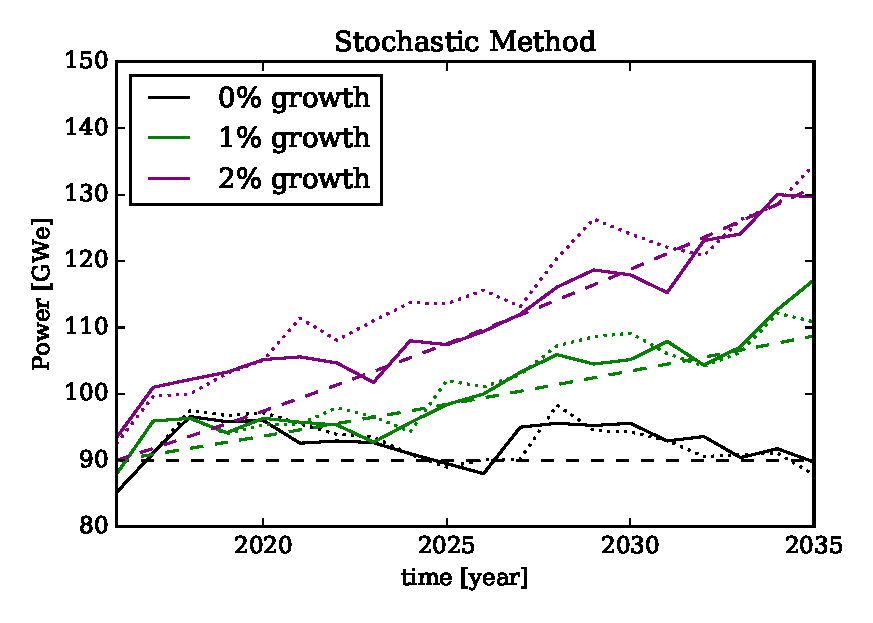
\includegraphics[width=0.9\textwidth]{demand-product-stochastic.eps}
\caption{Power production to demand comparison for 20 year deployment 
schedule optimization using only the \stochastic estimation method.
0\%, 1\%, and 2\% growth rates starting at 90 GWe are shown. Solid lines 
represent the bestguess deployment schedule.  Dotted lines are represent 
the second best guess deployment schedule. Dashed lines represent the 
demand curve that is targeted.
}
\label{demand-product-stochastic}
\end{figure}

